
\documentclass[10pt]{beamer}
\usepackage[utf8]{inputenc}

\usetheme[progressbar=frametitle]{metropolis}
\usepackage{appendixnumberbeamer}

\usepackage{booktabs}
\usepackage[scale=2]{ccicons}
\usepackage{verbatimbox}
\usepackage{pgfplots}
\usepackage{graphicx}
\setbeamercolor{background canvas}{bg=white}

\usepackage{xspace}
\newcommand{\themename}{\textbf{\textsc{metropolis}}\xspace}


\usepackage{amsmath}
\usepackage{nccmath}


\usepackage{makecell}
\renewcommand\theadalign{cb}
\renewcommand\theadfont{\bfseries}
\renewcommand\theadgape{\Gape[4pt]}
\renewcommand\cellgape{\Gape[4pt]}
\renewcommand\theadalign{cb}
\renewcommand\theadfont{\bfseries}
\renewcommand\theadgape{\Gape[4pt]}
\renewcommand\cellgape{\Gape[4pt]}


\title{Deep Learning Model for Base Calling of MinION Nanopore Reads}
%\subtitle{Master thesis assignment No. 1417}
% \date{\today}
\date{}
\author{Marko Ratković\\
Associate Profesor Mile Šikić, PhD}
\institute{University of Zagreb\\ Faculty of Electrical Engineering and Computing}
% \titlegraphic{\hfill\includegraphics[height=1.5cm]{logo.pdf}}

\begin{document}

\maketitle

%\begin{frame}{Table of contents}
%  \setbeamertemplate{section in toc}[sections numbered]
%  \tableofcontents[hideallsubsections]
%\end{frame}


%%%%%%%%%%%%%%%%%%%%%%%%%%%%%%%%%%%%%%%%%%%%%%%%%%%%%%%%%%%%%%%%%%%%%%%%%%%%%%%%%%%%%%%
%% FRAME
\begin{frame}[fragile]{MinION}
	\begin{figure}
		\begin{center}
			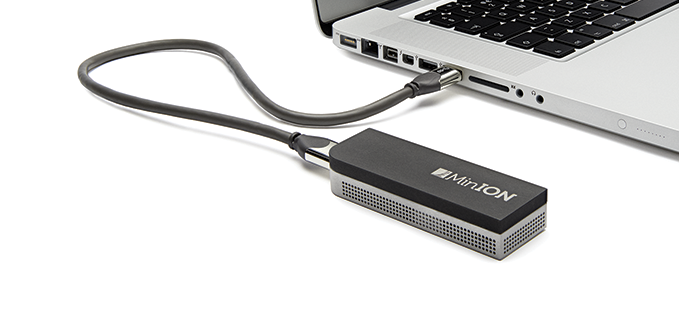
\includegraphics[width=1\textwidth]{imgs/minion.png}%
		    \caption{The MinION sequencing device}
		\end{center}
	\end{figure}
\end{frame}


%%%%%%%%%%%%%%%%%%%%%%%%%%%%%%%%%%%%%%%%%%%%%%%%%%%%%%%%%%%%%%%%%%%%%%%%%%%%%%%%%%%%%%%
%% FRAME
\begin{frame}[fragile]{Technology}
	\begin{figure}
		
		\begin{center}
			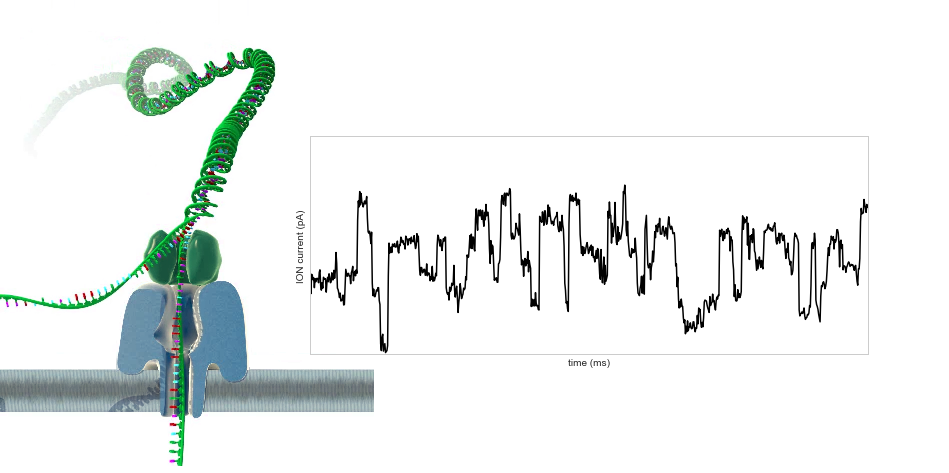
\includegraphics[width=1\textwidth]{imgs/nanopore_no_bases.png}%
			\caption{The MinION sequencing device}
		\end{center}
	\end{figure}
\end{frame}

%%%%%%%%%%%%%%%%%%%%%%%%%%%%%%%%%%%%%%%%%%%%%%%%%%%%%%%%%%%%%%%%%%%%%%%%%%%%%%%%%%%%%%%
%% FRAME
\begin{frame}[fragile]{Basecalling}
	\begin{figure}
		\begin{center}
			\includegraphics<1>[width=0.7\textwidth]{./imgs/basecall/basecall1.png}%
			\includegraphics<2>[width=0.7\textwidth]{./imgs/basecall/basecall2.png}%			
			\includegraphics<3>[width=0.7\textwidth]{./imgs/basecall/basecall3.png}%	
		\end{center}
	\end{figure}
\end{frame}

%%%%%%%%%%%%%%%%%%%%%%%%%%%%%%%%%%%%%%%%%%%%%%%%%%%%%%%%%%%%%%%%%%%%%%%%%%%%%%%%%%%%%%%
%% FRAME
\begin{frame}[fragile]{Basecalling options}

\alert{Metrichor}
\begin{itemize}
	\item only basecaller for ONT data
	\item proprietary software
	\item available as a cloud service
\end{itemize}

	\onslide<2> {
	\alert{Goals}
	\begin{itemize}
		\item local basecalling
		\item open-source
		\item speed, accuracy
	\end{itemize}
}

\end{frame}


%%%%%%%%%%%%%%%%%%%%%%%%%%%%%%%%%%%%%%%%%%%%%%%%%%%%%%%%%%%%%%%%%%%%%%%%%%%%%%%%%%%%%%%
%% FRAME
\begin{frame}[fragile]{Existing solutions}
	\begin{itemize}
		\item Third-party: \textit{DeepNano, NanoCall}
		\item Official: \textit{MinKNOW, Nanonet, Albacore, Scrappie}
	\end{itemize}
	\onslide<2->{
		\alert{Idea?}
		\begin{itemize}
		\item Signal segmentation – event detection
		\onslide<4->{\item RNN, HMM (older version of \textit{Metrichor} and \textit{NanoCall})}
		\end{itemize}
		
		
			\begin{figure}
				\begin{center}
					\includegraphics<2>[width=0.7\textwidth]{./imgs/segment/segmented_0.png}%
%					\includegraphics<3>[width=0.7\textwidth]{./imgs/segment/segmented_1.png}%			
%					\includegraphics<4>[width=0.7\textwidth]{./imgs/segment/segmented_2.png}%	
%					\includegraphics<5>[width=0.7\textwidth]{./imgs/segment/segmented_3.png}%			
%					\includegraphics<6>[width=0.7\textwidth]{./imgs/segment/segmented_4.png}%	
%					\includegraphics<7>[width=0.7\textwidth]{./imgs/segment/segmented_5.png}%
					\includegraphics<3->[width=0.7\textwidth]{./imgs/segment/segmented_full.png}%	
					\caption{Signal segmentation}			
				\end{center}
			\end{figure}
		
	}
\end{frame}


%%%%%%%%%%%%%%%%%%%%%%%%%%%%%%%%%%%%%%%%%%%%%%%%%%%%%%%%%%%%%%%%%%%%%%%%%%%%%%%%%%%%%%%
%% FRAME
\begin{frame}[fragile]{Proposed solution}
	\begin{center}  
		end2end
	\end{center}
\end{frame}


%%%%%%%%%%%%%%%%%%%%%%%%%%%%%%%%%%%%%%%%%%%%%%%%%%%%%%%%%%%%%%%%%%%%%%%%%%%%%%%%%%%%%%%
%% FRAME
\begin{frame}[fragile]{Models}
	\only<1>{
		\begin{figure}
			\begin{center}
				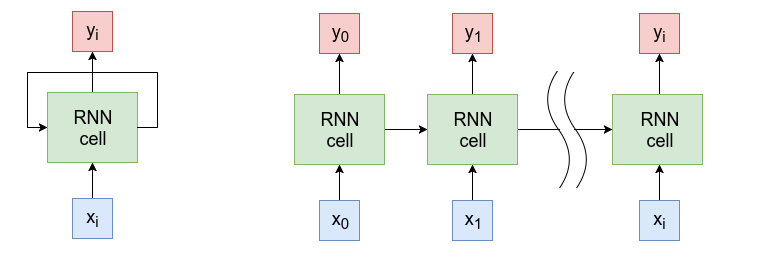
\includegraphics[width=0.8\textwidth]{./imgs/model/rnn.png}%	
				\caption{RNN}
			\end{center}
		\end{figure}	
	}
	\addtocounter{figure}{1}
	\only<2>{
		\begin{figure}
			\begin{center}
				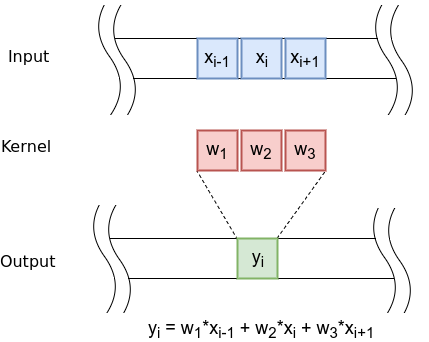
\includegraphics[width=0.6\textwidth]{./imgs/model/convolution.png}%	
				\caption{CNN}
			\end{center}
		\end{figure}
	}
	\addtocounter{figure}{1}
	\only<3>{
		\begin{figure}
			\begin{center}
				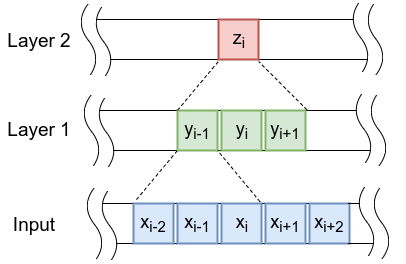
\includegraphics[width=0.7\textwidth]{./imgs/model/receptive_field.png}%	
				\caption{Receptive field}
			\end{center}
		\end{figure}
	}
\end{frame}

%%%%%%%%%%%%%%%%%%%%%%%%%%%%%%%%%%%%%%%%%%%%%%%%%%%%%%%%%%%%%%%%%%%%%%%%%%%%%%%%%%%%%%%
%% FRAME
\begin{frame}[fragile]{CTC loss}
	\alert{Idea}: decode sequence from fixed-width output (softmax over alphabet)
	\only<2>{
		\begin{figure}
			\begin{center}
				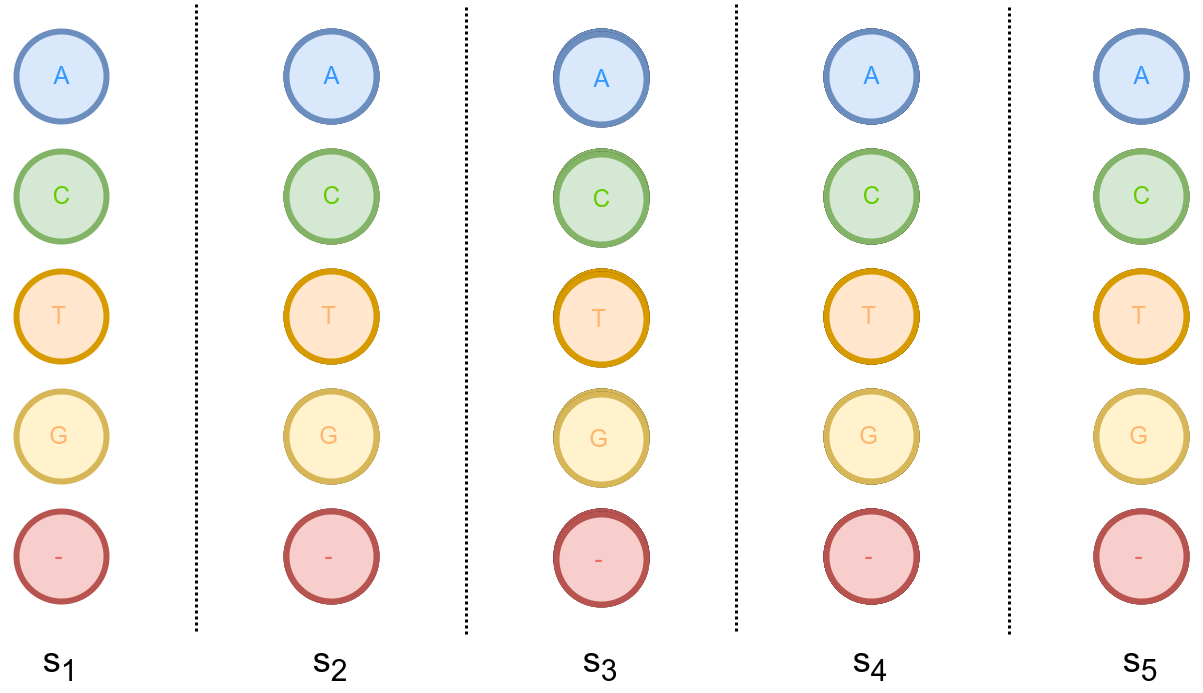
\includegraphics[width=0.7\textwidth]{./imgs/ctc/graph_0.png}%	
				\caption{Output}
			\end{center}
		\end{figure}	
	}
	\only<3->{
		\addtocounter{figure}{1}
		\begin{figure}
			\begin{center}
				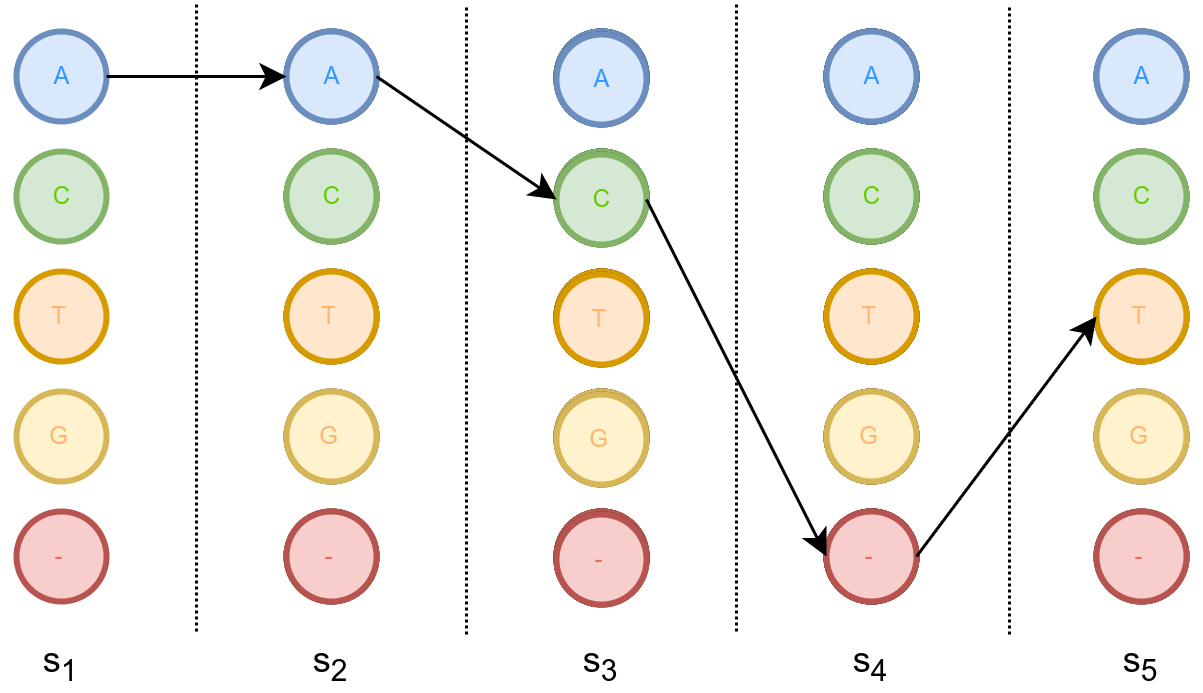
\includegraphics[width=0.7\textwidth]{./imgs/ctc/graph_1.png}%	
				\caption{Path "AAC-T"}
			\end{center}
		\end{figure}
	}
	
	
	\onslide<3->{
		\begin{equation}
		\begin{gathered}
			P(\pi | X) = \prod_{t=1}^{m} s_t(\pi_t)
		\end{gathered}
		\end{equation}
	}
\end{frame}

%%%%%%%%%%%%%%%%%%%%%%%%%%%%%%%%%%%%%%%%%%%%%%%%%%%%%%%%%%%%%%%%%%%%%%%%%%%%%%%%%%%%%%%
%% FRAME
\begin{frame}[fragile]{CTC loss}
	\alert{Idea}: decode sequence from fixed-width output
	\onslide<2->{
		\begin{equation}
			\begin{gathered}
			\label{eq:multiple}
			ACT = \begin{cases}
			decode(A, A, A, C, T) \\
			decode(A, A, C, -, T) \\
			decode(-, A, C, T, T)  \\
			decode(-, -, A, C, T)  \\
			decode(A, C, C, C, T)  \\
			\vdots \\
			decode(A, C, T, -, -) 
			\end{cases}
			\end{gathered}
		\end{equation}
	}
	\onslide<3->{	
		\begin{equation}
			\begin{gathered}
			P(Y | X) = \sum_{\pi \in decode^{-1}(Y)}^{} P(\pi | X)
			\end{gathered}
		\end{equation}
	}
\end{frame}

%%%%%%%%%%%%%%%%%%%%%%%%%%%%%%%%%%%%%%%%%%%%%%%%%%%%%%%%%%%%%%%%%%%%%%%%%%%%%%%%%%%%%%%
%% FRAME
\begin{frame}[fragile]{CTC loss}

Given the dataset $D = \{(X_i, Y_i)\}$, training objective is the maximization of the likelihood of each training sample  which is the same as the minimization of negative log likelihood:

	\begin{equation}
		\begin{gathered}
		L(D) = - \sum_{(X,Y)\in D}^{} ln P(Y | X)
		\end{gathered}
	\end{equation}
		
\end{frame}
%%%%%%%%%%%%%%%%%%%%%%%%%%%%%%%%%%%%%%%%%%%%%%%%%%%%%%%%%%%%%%%%%%%%%%%%%%%%%%%%%%%%%%%
%% FRAME
\begin{frame}[fragile]{Training data}
		
	\begin{figure}
		\begin{center}
			\includegraphics<1>[width=1\textwidth]{./imgs/train/t1.png}%
			\includegraphics<2>[width=1\textwidth]{./imgs/train/t2.png}%
			\includegraphics<3>[width=1\textwidth]{./imgs/train/t3.png}%
			\includegraphics<4>[width=1\textwidth]{./imgs/train/t4.png}%
			\includegraphics<5>[width=1\textwidth]{./imgs/train/t5.png}%
			\caption{Dataset preparation}
		\end{center}
	\end{figure}
\end{frame}

%%%%%%%%%%%%%%%%%%%%%%%%%%%%%%%%%%%%%%%%%%%%%%%%%%%%%%%%%%%%%%%%%%%%%%%%%%%%%%%%%%%%%%%
%% FRAME
%\begin{frame}[fragile]{Training data}
%	\begin{figure}
%		\begin{center}
%			
\includegraphics[width=0.7\textwidth]{./imgs/preprocess.png}%
%			\caption{Preprocess}
%		\end{center}
%	\end{figure}
%\end{frame}

%%%%%%%%%%%%%%%%%%%%%%%%%%%%%%%%%%%%%%%%%%%%%%%%%%%%%%%%%%%%%%%%%%%%%%%%%%%%%%%%%%%%%%%
%% FRAME
\begin{frame}[fragile]{Status}
 	\begin{itemize}
	\item Loss 
	\item Dataset
	\item \alert{Model? CNN?}
\end{itemize}
\end{frame}

%%%%%%%%%%%%%%%%%%%%%%%%%%%%%%%%%%%%%%%%%%%%%%%%%%%%%%%%%%%%%%%%%%%%%%%%%%%%%%%%%%%%%%%
%% FRAME
\begin{frame}[fragile]{Model}
	\begin{itemize}
		\item<1-> Residual CNN
		\item<2-> 72 blocks, 2M parameters
		\item<3-> Maxpool every 24 blocks, reduction of dimensionality by factor 8
	\end{itemize}
	\onslide<2-> {
		\begin{figure}
			\begin{center}
				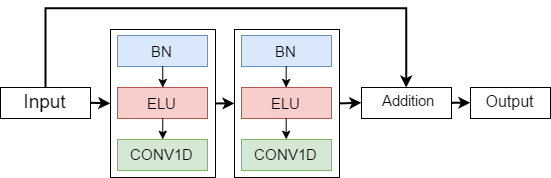
\includegraphics[width=0.7\textwidth]{./imgs/model/block_small.png}%
				\caption{Residual block}	
			\end{center}
		\end{figure}
	}
\end{frame}


%%%%%%%%%%%%%%%%%%%%%%%%%%%%%%%%%%%%%%%%%%%%%%%%%%%%%%%%%%%%%%%%%%%%%%%%%%%%%%%%%%%%%%%
%% SECTION 
\section{Results}
%%%%%%%%%%%%%%%%%%%%%%%%%%%%%%%%%%%%%%%%%%%%%%%%%%%%%%%%%%%%%%%%%%%%%%%%%%%%%%%%%%%%%%%
%% FRAME
\begin{frame}[fragile]{Results}	
	\begin{figure}[!htb]
		\begin{center}
			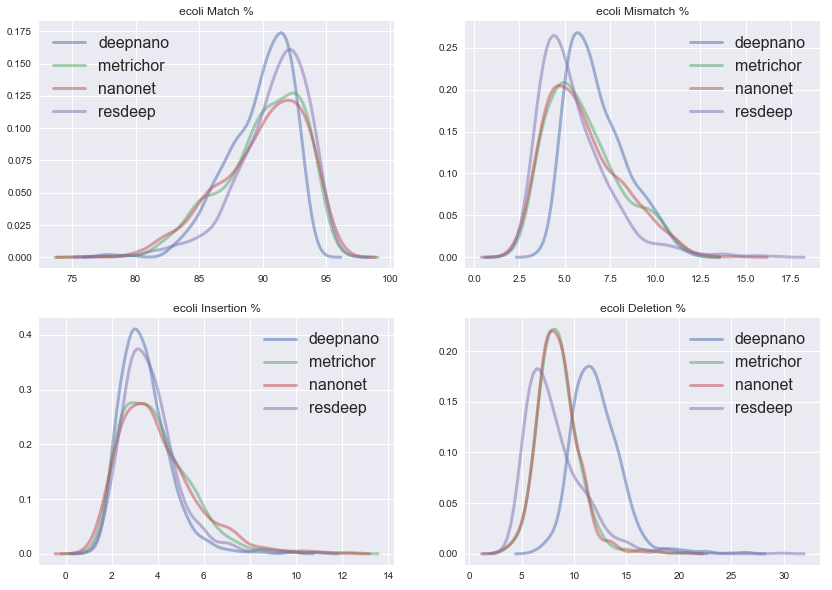
\includegraphics[width=0.8\textwidth]{imgs/results/kde_cigar.png}
			\caption{KDE plot of alimnment operations for E. Coli}
			\label{fg:consensus}
		\end{center}
	\end{figure}
\end{frame}


%%%%%%%%%%%%%%%%%%%%%%%%%%%%%%%%%%%%%%%%%%%%%%%%%%%%%%%%%%%%%%%%%%%%%%%%%%%%%%%%%%%%%%%
%% FRAME
\begin{frame}[fragile]{Results}
	\begin{table}[htbp]
		\caption{Alignment specifications of E. Coli R9 basecalled reads}
		\label{tbl:ecoli_rates}
		\centering
		\begin{tabular}{lcccc}
			\toprule
			{} &  \thead{Match \% \\(median)} &  \thead{Mismatch \% \\(median)} &  \thead{Insertion \% \\(median)} &  \thead{Deletion \% \\(median)} \\
			\midrule
			DeepNano   &                  90.254762 &                      6.452852 &                       \textbf{3.274420} &                     11.829965 \\
			Metrichor  &                  90.560455 &                      5.688105 &                       3.660381 &                      8.328271 \\
			Nanonet    &                  90.607674 &                      5.608912 &                       3.652791 &                      8.299046 \\
			resdeep    &                  \textbf{91.408591} &                     \textbf{ 5.019141} &                       3.477739 &                      \textbf{7.471608 }\\
			\bottomrule
		\end{tabular}
	\end{table}
	
\end{frame}

%%%%%%%%%%%%%%%%%%%%%%%%%%%%%%%%%%%%%%%%%%%%%%%%%%%%%%%%%%%%%%%%%%%%%%%%%%%%%%%%%%%%%%%
%% FRAME
\begin{frame}[fragile]{Results}
\begin{table}[htb]
	\caption{Ecoli R9 basecalled read lengths in base pairs}
	\label{tbl:ecoli_lens}
	\centering
	
	\begin{tabular}{lccc}
		\toprule
		{} &  \thead{median} &   \thead{mean} &    \thead{std} \\
		\midrule
		DeepNano   &        5526.5 &  8126.694000 &  7406.554786 \\
		Metrichor  &        5809.5 &  8933.275000 &  9189.709720 \\
		Nanonet    &        3286.5 &  4874.406582 &  4803.182344 \\
		resdeep    &        5784.0 &  8990.988989 &  9297.972688 \\
		\bottomrule
	\end{tabular}
\end{table}
	
\end{frame}
%%%%%%%%%%%%%%%%%%%%%%%%%%%%%%%%%%%%%%%%%%%%%%%%%%%%%%%%%%%%%%%%%%%%%%%%%%%%%%%%%%%%%%%
%% FRAME
\begin{frame}[fragile]{Results}
	\alert{Consensus from pileup}
	
	\only<1> {
		\begin{figure}[!htb]
			\begin{center}
				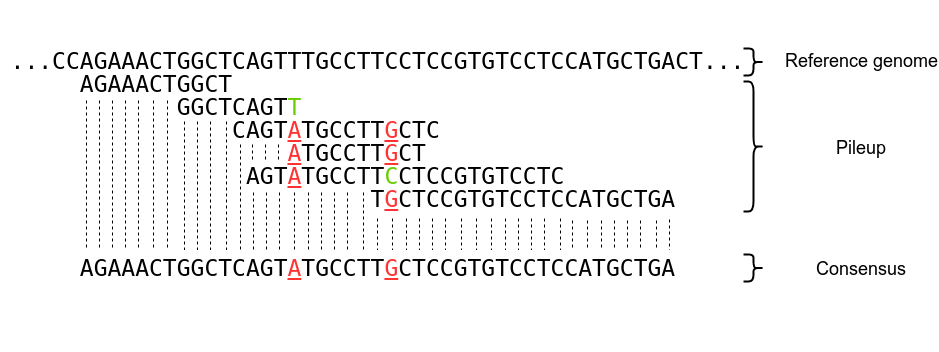
\includegraphics[width=0.8\textwidth]{imgs/consnesus.png}
				\caption{Consensus from pileup}
				\label{fg:consensus}
			\end{center}
		\end{figure}
	}
	\only<2> {
		\begin{table}[!htb]
			\caption{Consensus specification of E. Coli R9 basecalled reads}
			\label{tbl:spec_ecoli}
			\centering
			\centering \small%
			\resizebox{\textwidth}{!}{
				\begin{tabular}{lcccccc}
					\toprule
					{} &  \thead{Match\\\%} &  \thead{Snp\\\%} &  \thead{Insertion\\\%} &  \thead{Deletion\\\%} \\
					\midrule
					DeepNano  &            98.8742 &         1.0044 &               0.1214 &              0.9041 \\
					Metrichor &            99.1223 &         0.7464 &               0.1313 &              0.6300 \\
					Nanonet   &            97.9691 &         1.5700 &               0.4609 &              1.5158 \\
					resdeep   &     \textbf{99.2361} &         \textbf{0.6474} &               \textbf{0.1165} &             \textbf{ 0.5510 }\\
					\bottomrule
				\end{tabular}
			}
		\end{table}
	}
	
\end{frame}

%%%%%%%%%%%%%%%%%%%%%%%%%%%%%%%%%%%%%%%%%%%%%%%%%%%%%%%%%%%%%%%%%%%%%%%%%%%%%%%%%%%%%%%
%% FRAME
\begin{frame}[fragile]{Results}
\alert{Consensus from de novo assembly} obtained using assembler \emph{ra}\footnote{\url{https://github.com/rvaser/ra}} and compared to the reference using \textit{dnadiff} present in the Mumer\footnote{\url{https://github.com/garviz/MUMmer}}

\onslide<2->{
	\begin{table}[htb]
		\caption{Assembly and consensus results for E. Coli}
		\label{tbl:assembly}
		\centering \small%
	   	\resizebox{\textwidth}{!}{
	   		
	   		\begin{tabular}{lccc}
	   			\toprule
	   			&         \thead{Metrichor} &           \thead{resdeep} &    \thead{Nanonet} \\
	   			\midrule
	   			% \thead{Ref. genome size (bp)} &           4639675 &           4639675 &            4639675 \\
	   			% \thead{Total bases (bp)}      &           4604806 &           \textbf{4614354} &          4600056 \\
	   			% \thead{Contigs [\#]}           &                 1 &                 1 &                1 \\
	   			\thead{Aln. bases ref. (bp)}  &  4639641(100.00\%) &  4639612(100.00\%) &  4639031(99.99\%) \\
	   			\thead{Aln. bases query (bp)} &  4604787(100.00\%) &  4614351(100.00\%) &  4599745(99.99\%) \\
	   			\thead{Avg. Identity}         &             98.76 &             \textbf{99.06} &            98.47 \\
	   			\thead{Edit distance}         &             60418 &             \textbf{46686 }&            74341 \\
	   			\bottomrule
	   		\end{tabular}
	   	}
	\end{table}
}
\end{frame}

%%%%%%%%%%%%%%%%%%%%%%%%%%%%%%%%%%%%%%%%%%%%%%%%%%%%%%%%%%%%%%%%%%%%%%%%%%%%%%%%%%%%%%%
%% FRAME
\begin{frame}[fragile]{Results - basecalling speed}
\begin{table}[htbp]

	\caption{Base calling speeds measured in \textit{base pairs per second}\footnote{Tested on server with two 8-core Intel(R) Xeon(R) E5-2640 v2 CPUs, NVIDIA Titan Black GPU, 6GB}}
	\label{tbl:speeds}
	
	\centering
	\begin{tabular}{lccc}
		\toprule
		{} &  \thead{resdeep} &  \thead{Nanonet} &  \thead{DeepNano}  \\
		\midrule
		Speed CPU(bp/s)  & \textbf{ 1363.34 } & 897.49 & 692.37 \\
		Speed GPU(bp/s)  & \textbf{ 6571.76 } & 3828.39  & - \\
		\bottomrule
	\end{tabular}
	

\end{table}	
\end{frame}

%%%%%%%%%%%%%%%%%%%%%%%%%%%%%%%%%%%%%%%%%%%%%%%%%%%%%%%%%%%%%%%%%%%%%%%%%%%%%%%%%%%%%%%
%% FRAME
\begin{frame}[fragile]{Conclusion}
	\begin{itemize}
		\item end2end basecaller, open-source, fast and accurate
		\item \alert{Note:} R9 data only, R9.4 in progress
	\end{itemize}
\end{frame}

%%%%%%%%%%%%%%%%%%%%%%%%%%%%%%%%%%%%%%%%%%%%%%%%%%%%%%%%%%%%%%%%%%%%%%%%%%%%%%%%%%%%%%%
%% FRAME
\begin{frame}[fragile]{Future work}
	\begin{itemize}
		\item<1-> Scaled Exponential Linear Units (SELU), Jun 2017
		\item<3-> Facebook AI Research (FAIR) team: \textit{Convolutional Sequence to Sequence Learning}, May 2017
		\item<4-> ...
	\end{itemize}
	
	\onslide<2> {
		\begin{figure}

			\begin{center}
				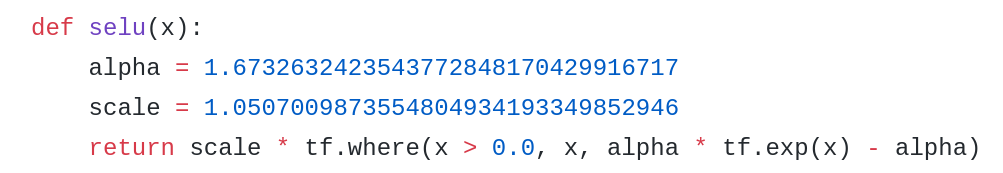
\includegraphics[width=0.9\textwidth]{./imgs/selu_tf_exp.png}%
				\caption{SELU implementation}				
			\end{center}
		\end{figure}
	}
\end{frame}

%%%%%%%%%%%%%%%%%%%%%%%%%%%%%%%%%%%%%%%%%%%%%%%%%%%%%%%%%%%%%%%%%%%%%%%%%%%%%%%%%%%%%%%
%% FRAME

\begin{frame}[standout]
	Questions?
\end{frame}	


\end{document}
